% Diffuse Correlation Spectroscopy 

%% Objective and Theory 
%%% Replicate the temporal autocorrelation measurements from Wayne et.al. (2023)
%%% Single pixel autocorrelation model g(2) = n n(\tau) / n^2
%%% Ensable (spatial) average formula to combine pixels. 

%% Experimental Setup 
%%% Params: 785 nm, 60 mW, 
%%% SPAD: 125 um, Z_SPAD 10 mm Z_laser 150 mm , geometry, DCR,
%%% Datarates, 150 kps, at a int time, results in certain number of counts, which need to be sent to the computer. Limit from swiabian, limit from PC?
%%% Measured spot size? 

%% Measurement Procedure
%%% Binwidth and n_bins define the total window. 
%%% Three diffuser speeds. 

%% Results 
%%% Decorrelation times vs Diffuser speed. 
%%% Noise Reduction and averaging. 

\subsection{3rd Measurement: Diffuse Correlation Spectroscopy}

As seen in the second measurement, true thermal light decorrelates in femtoseconds, which is too fast for the SPAD dead time to measure. 
To address this, we utilized a pseudo-thermal light source. 
The experiment shines the 785 nm continuous-wave (CW) laser through a rotating diffuser to generate a dynamic speckle pattern. 
The formula for the average speckle diameter $S \approx 1.22 \lambda z_{det} / D$, where $z_{det}$ is the distance from the diffuser to the detector plane, yields an estimated speckle diameter of $1.58\ \mu\text{m}$ for our particular setup.\footnote{Assuming a uniform circular scattering spot, an operating wavelength of $785\text{ nm}$, and perfect laser alignment spanning exactly half of the diffuser's diameter (i.e an illumination spot size of $D = 22.7\text{ mm}$).}.
By changing the motor speed, this moving diffuser creates macroscopic intensity fluctuations in the millisecond regime, allowing our Time Tagger to capture the decorrelation dynamics.

\begin{figure}[h!]
    \centering 
    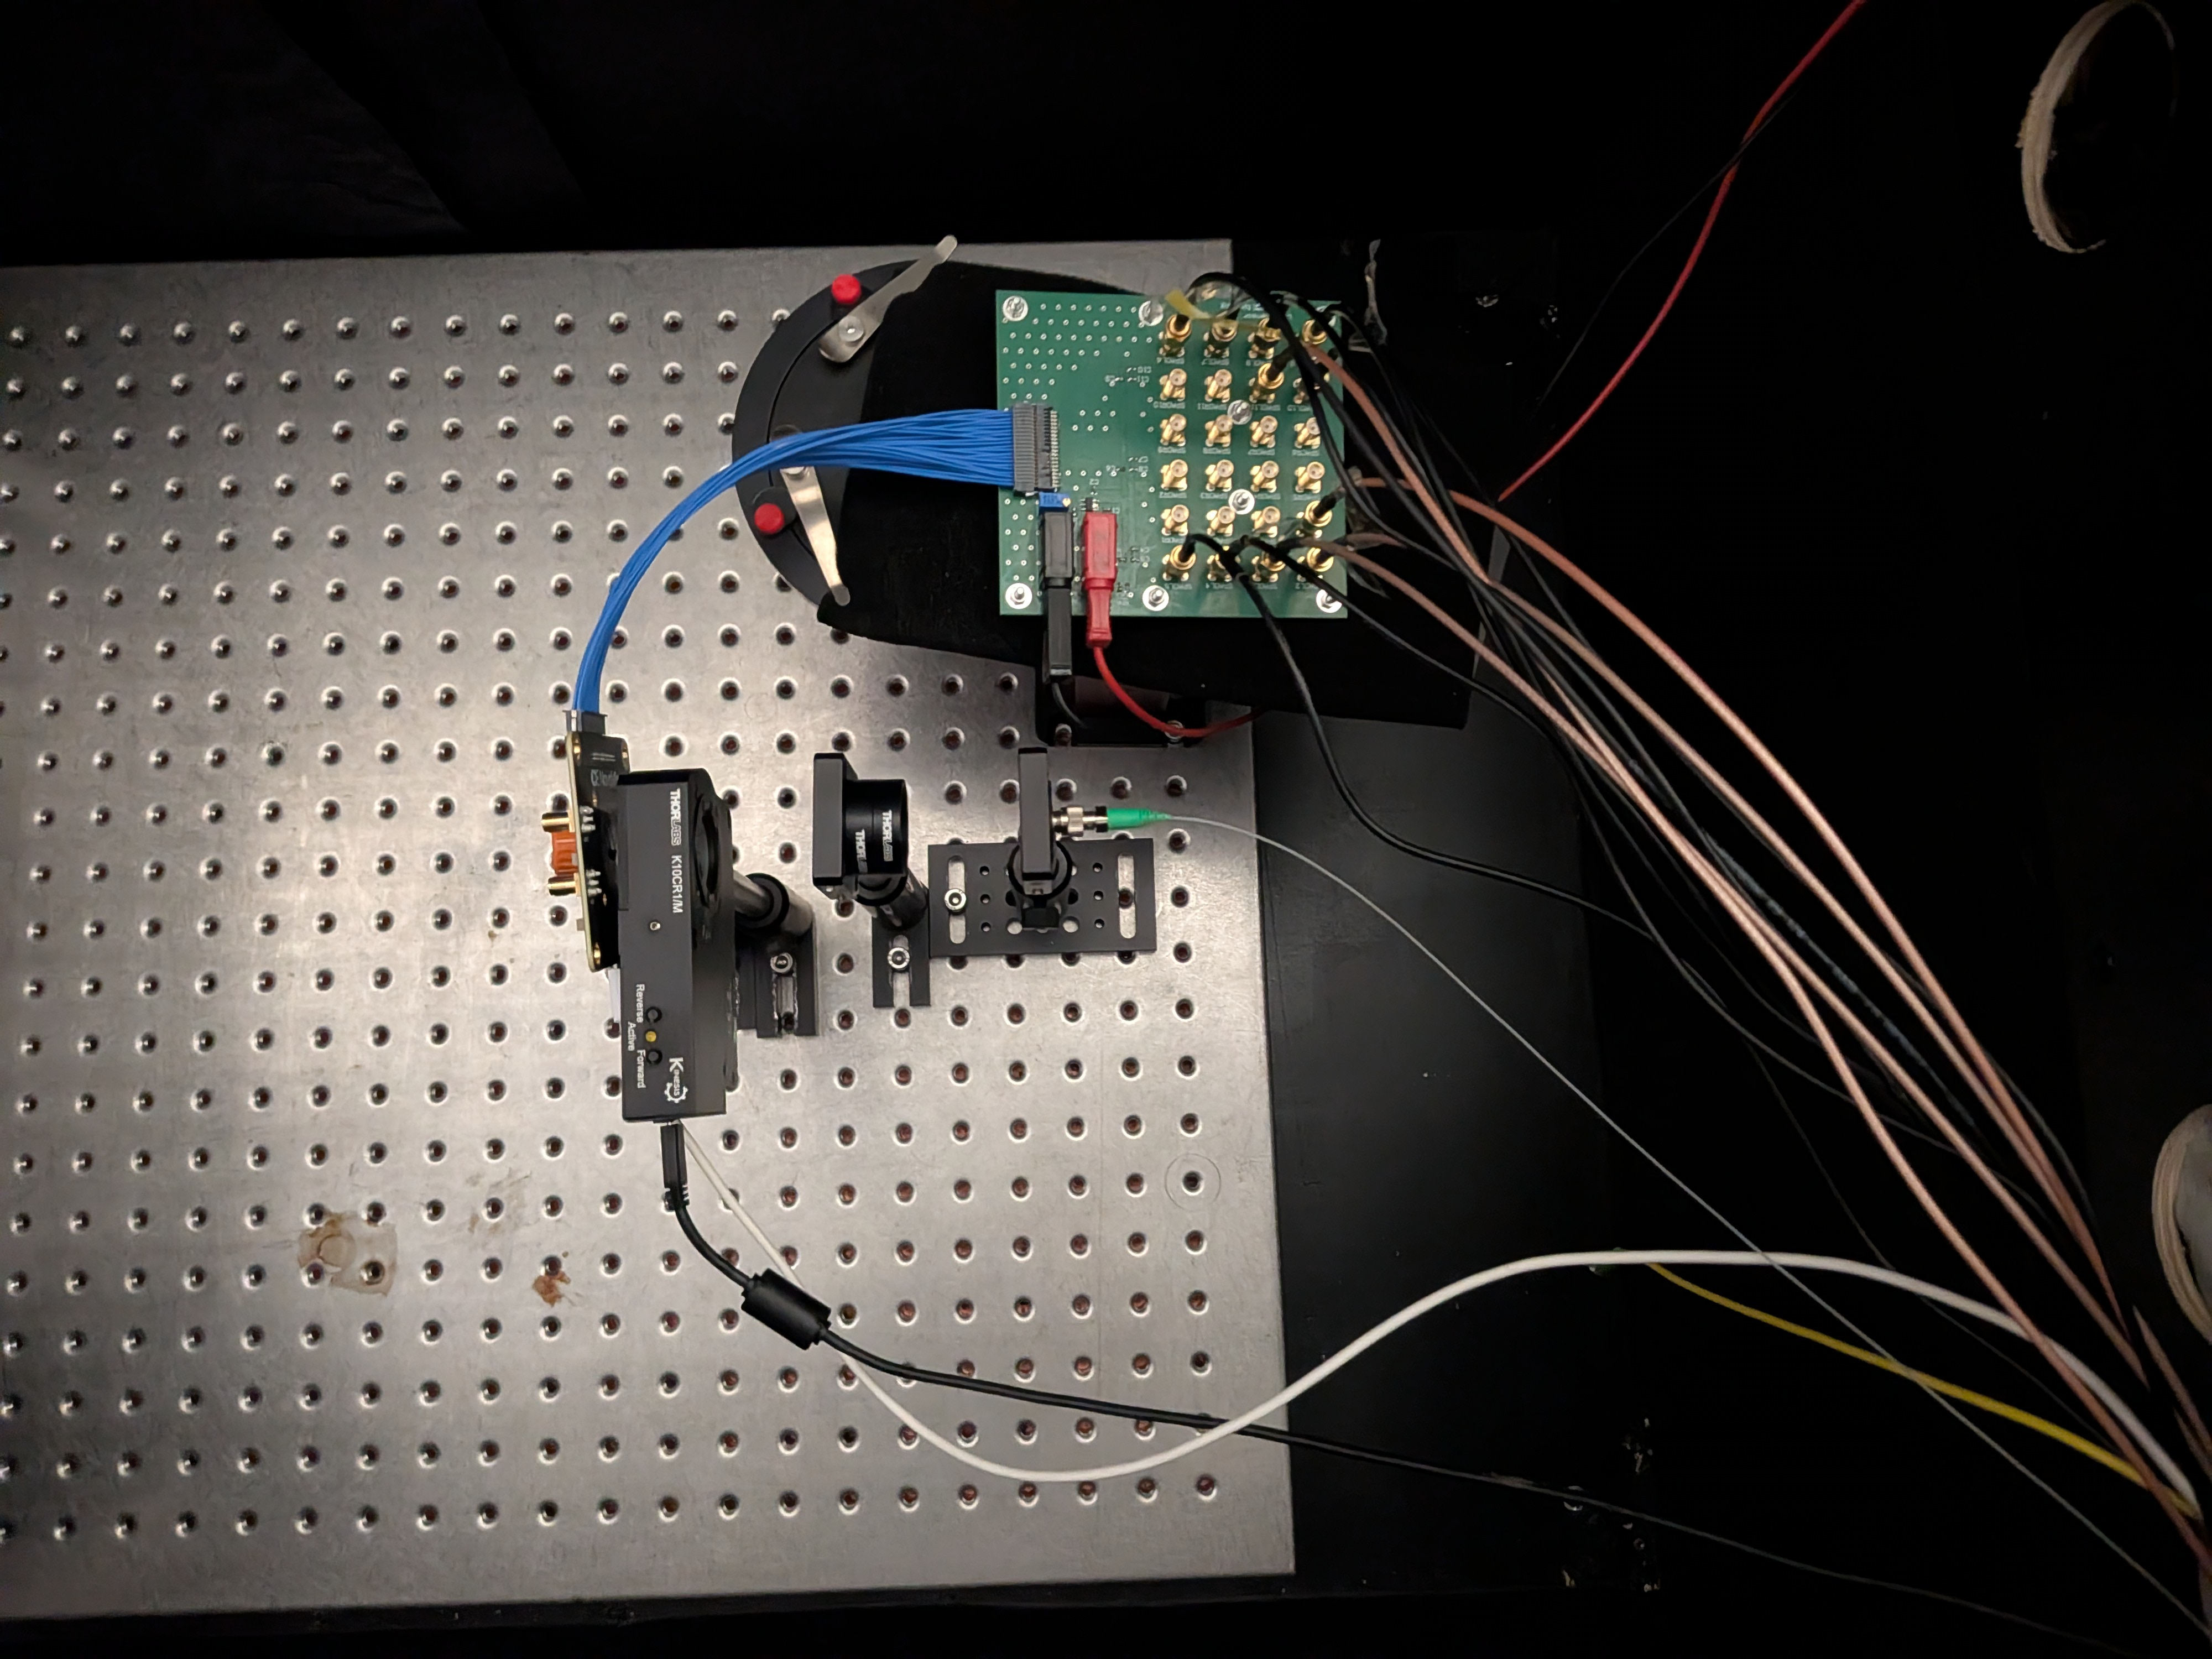
\includegraphics[width = 0.45 \textwidth]{Figures/PXL_20260611_192951368.MP.jpg}
    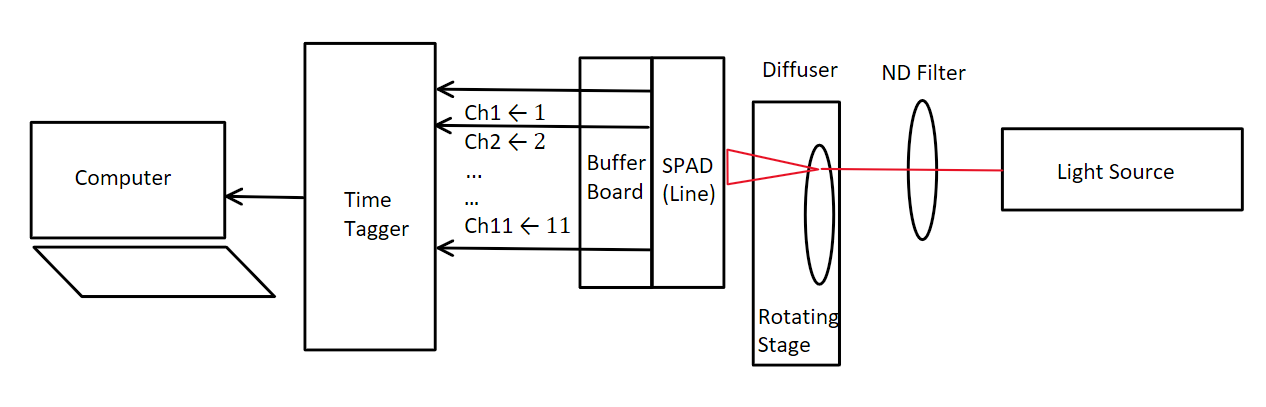
\includegraphics[width=0.45\textwidth]{Figures/exp_layout2_diagram.png}
    \caption{Dynamic speckle setup measurement. CW laser incident onto the rotating diffuser with the SPAD detector array positioned behind it (left).}
\end{figure}

The measurement procedure was as follows:
\begin{enumerate}
    \item A 785 nm CW laser was aligned to hit the right edge of a rotating diffuser.
    \item The line sensor SPAD array was placed at a distance $z_{det}=37.5\text{ mm}$ behind the diffuser to detect the speckles.
    \item To avoid hardware buffer overflow from high count rates, we lowered the laser intensity to a safe kilocounts-per-second (kcps) level.
    \item To recover the signal-to-noise ratio (SNR), we simultaneously measured the autocorrelation of 11 separate pixels to average them together.
    \item The measurement was repeated for different diffuser angular velocities (5, 10, 15, and 20 deg/s).
\end{enumerate}

\textbf{Results} \\
To process the data, each pixel's measurement was normalized by dividing it by its flat baseline. Figure \ref{fig:dcs_average_fit} shows the 11 individual pixels (faded) and their combined average (black). Averaging the pixels gives a much smoother exponential decay curve, allowing us to accurately fit the data and extract the decorrelation time ($\tau_c$). The data was fitted using the standard intensity correlation model:

$$g^{(2)}(\tau) = 1 + \beta \exp\left(-2\frac{\tau}{\tau_c}\right)$$

where $\beta$ is the spatial coherence factor and $\tau_c$ is the characteristic decorrelation time.

\begin{figure}[H]
    \centering
    
\includegraphics[width=0.5\textwidth]{figures/average11_decorrelation_spectroscopy.png}
    \caption{Normalized autocorrelation measurement for the rotating diffuser. The black line is the average of 11 pixels, which is fitted with an exponential curve (red dashed line) to extract $\tau_c$.}
    \label{fig:dcs_average_fit}
\end{figure}

Figure \ref{fig:spatial_averaging} demonstrates why using the 11-pixel array brings an advantage. 
As we average more pixels ($N$), the measured decorrelation time remains stable, but the baseline noise drops following the theoretical $1/\sqrt{N}$ rule. 

\begin{figure}[h!]
    \centering
    
\includegraphics[width=0.5\textwidth]{figures/averageeffect_decorrelation_spectroscopy.png}
    \caption{Effect of averaging multiple pixels. The measured $\tau_c$ remains stable (Left), while the noise drops with $1/\sqrt{N}$ (Right).}
    \label{fig:spatial_averaging}
\end{figure}

Finally, Figure \ref{fig:velocity_sweep} plots the extracted $\tau_c$ against the different motor speeds. 
As the diffuser spins faster, the speckles move past the detector faster, causing the decorrelation time to drop. 
This inverse relationship is consistent with this proof-of-principle demonstration of Diffuse Correlation Spectroscopy (DCS) using a the pseudo-thermal source.

\begin{figure}[h!]
    \centering
    
\includegraphics[width=0.5\textwidth]{figures/average11_decorrelation_spectroscopy_differentspeeds.png}
    \caption{Decorrelation time ($\tau_c$) measured at different diffuser speeds. As angular velocity increases, $\tau_c$ proportionally decreases.}
    \label{fig:velocity_sweep}
\end{figure}